\documentclass[a4paper]{article}   

\usepackage[utf8]{inputenc}
\usepackage[english]{babel}

\usepackage{tikz}
\usepackage{verbatim}

% \usepackage{multirow}

% \usepackage{graphicx}
% \usepackage{algorithmic}
% \usepackage{amsmath}
\usepackage{hyperref}

% \usepackage[french]{algorithm2e}

% \usepackage{enumerate}

\title{Co-reference Resolution}
\author{Yohan Chalier}
\date{\today}

\renewcommand{\arraystretch}{1.2}

\begin{document}

\begin{titlepage}
	\centering
	\vspace{1cm}
	{\scshape\LARGE Télécom ParisTech \par}
	\vspace{1cm}
	{\scshape\Large Symbolic Natural Language Processing (SD213) \par}
	\vspace{1.5cm}
	{\huge\bfseries Co-reference resolution\par}
	\vspace{2cm}
	{\Large\itshape Yohan Chalier \par}
	\vfill

% Bottom of the page
	{\large \today\par}
\end{titlepage}


\begin{abstract}

\end{abstract}

\section{Problem positioning}

\paragraph{What is co-reference?}

\emph{Co-reference} occurs when two or more expressions refers to the same referent. Usually, one expression is in a full form (the \emph{antecedent}) and the other one in a abbreviated form (a \emph{proform}).

~\par

For example:

\textit{The \textbf{music} was so loud that \textbf{it} couldn't be enjoyed.}

~\par

Co-reference resolution is needed to derive a correct interpretation of a text.

\paragraph{The problem of co-reference resolution}

\paragraph{Naive algorithm}
Look for the nearest preceding individual that is compatible with the referring expression.

~\par

It solves sentences like this:

{\em \hspace{\parindent} The girl\textsubscript{1} likes her\textsubscript{1} brother\textsubscript{2} and protects him\textsubscript{2}.}

~\par

But it fails to differentiate those sentences:

{\em \hspace{\parindent} He\textsubscript{?} said that John\textsubscript{?} was coming.}

{\em \hspace{\parindent} His\textsubscript{1} sister said that John\textsubscript{1} was coming.}

\paragraph{Domination and c-command}

\paragraph{Domination}
Node $N_1$ dominates node $N_2$ if $N_1$ is above $N_2$ in the tree and one can trace a path from $N_1$ to $N_2$ moving only downwards in the tree (never upwards).

\paragraph{c-command}
Node $N_1$ c-commands node $N_2$ if
\begin{itemize}
\item $N_1$ does not dominate $N_2$
\item $N_2$ does not dominate $N_1$
\item The first (i.e. the lowest) branching node that dominates $N_1$ also dominates $N_2$
\end{itemize}

\paragraph{Domination and c-command}

\begin{center}
\begin{tikzpicture}
\node{M}
	child {node {A}}
	child {node {B}
		child {node {C} child {node {E}}}
		child {node {D}
			child {node {F}}
			child {node {G}}
		}
	};
\end{tikzpicture}
\end{center}

\paragraph{Co-reference and c-command}

It was hypothesized that one restriction between proform and antecedent is that {\bfseries the proform cannot appear in a position where it \emph{c-commands} its antecedent}.

~\par

This is not trivial: Bouchard, Denis. (2010). \textit{Une explication cognitive des effets attribués à la c-commande dans les contraintes sur la coréférence}. Corela. 10.4000/corela.965.

\paragraph{When John Comes Marching Home}

\emph{he} said that \emph{john} was coming

\begin{figure}
\centering
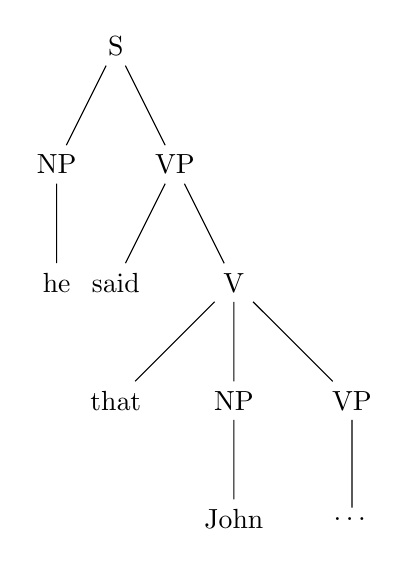
\begin{tikzpicture}
\node{S}
	child {node {NP}
		child {node {he}}		
		}
	child {node {VP}
		child {node {said}}
		child {node {V}
			child {node {that}}
			child {node {NP}
				child {node {John}}
			}
			child {node {VP}
				child {node {\ldots}}			
			}
		}
	};
\end{tikzpicture}
\end{figure}

\emph{his} mother said that \emph{john} was coming

\begin{center}
\begin{tikzpicture}
\node{S}
	child {node[left=1cm] {NP}
		child {node {his}}
		child {node {mother}}
	}
	child {node {VP}
		child {node {said}}
		child {node {V}
			child {node {that}}
			child {node {NP}
				child {node {John}}
			}
			child {node {VP}
				child {node {\ldots}}			
			}
		}
	};
\end{tikzpicture}
\end{center}

\section{Implementation}

\paragraph{Current implementation}

A Python script that contains:

\begin{itemize}
\item a small grammar and lexicon
\item a very basic top-down parser in a class \texttt{Parser}
\item a \texttt{Node} class to represent a syntax tree
\end{itemize}

\paragraph{Co-reference resolution}
For each word recognized as a referring expression (for now, only pronouns), a method of the \texttt{Parser} finds a compatible word (\emph{features agreement}), and if the proform does not c-command that word, it links them both.

\paragraph{See it in action}

\begin{verbatim}
Parsing: he said that John was_coming

 |_ s
   |_ np
     |_ pn : he
   |_ vp
     |_ v : said
     |_ sub
       |_ p : that
       |_ n : John
       |_ v : was_coming

he_0 said that John was_coming
\end{verbatim}

\begin{verbatim}
Parsing: his sister said that John was_coming
his_0 sister said that John_0 was_coming

Parsing: the girl likes her brother and protects him
the girl_0 likes her_0 brother_1 and protects him_1
\end{verbatim}

\paragraph{Difficulties and perspectives}

\begin{itemize}
\item Parser improvement (if time, use CKY)
\item Use more features to check compatibility (now just 2)
\item Perform more tests to compute a precision score
\item Ultimately, try parsing several sentences to find references across sentences
\end{itemize}

~\par

The script is available on GitHub:

\url{https://github.com/ychalier/coref/}


\begin{thebibliography}{9}

\end{thebibliography}

\listoffigures

\listoftables

\end{document}
